\documentclass[main.tex]{subfiles}

\theoremstyle{definition}
\newtheorem{definition}{Definition}[section]

\begin{document}
\section{Grover's algorithm}
In this section we will discuss about Grover's algorithm and its 
utilisation in the MST problem.
We can start with its definition,
\theoremstyle{definition}
	\begin{definition}{\textbf{Grover's algorithm}}
	Grover's algorithm is a quantum algorithm that finds with high 
	probability the input to a black box function that produces a 
	particular output value.
	$$f:\{0, 1, ..., N-1\}\rightarrow\{0,1\},\quad where \quad N=2^{n}\textit{, }n\in\mathbb{N}$$ 
	\[
    f(x)=\left\{
                \begin{array}{ll}
                  0 \quad\text{if }x \neq w\\
                  1 \quad\text{if }x = w
                \end{array}
              \right.
  \]
	\end{definition}
	
	\subsection{Algorithm characteristics}
The applications of the algorithm can be many, but usually, as it is presented in the original paper of Grover, the algorithm
is described as "searching a database". This definition is not really precise inasmuch the algorithm cannot be used for actual databases (see https://web.eecs.umich.edu/~imarkov/pubs/jour/cise05-grov.pdf, \textit{Hint}: construct an oracle for an unstructured database have a linear complexity, this will be clear in a moment). As we have said in the definition, if we have $y=f(x)$ the algorithm can calculates efficiently $x$ when given $y$.
Inverting a function is related to the searching of a database because we could come up with a function that produces one particular value of $y$ (1, for instance) if $x$ matches a desired entry in a database, and another value of $y$ (0) for other values of $x$. So Grover's algorithm can be seen as a searching algorithm in an unstructured table.
Now let's analyse the definition step by step. 

Like many quantum algorithms, Grover's algorithm is probabilistic in the sense that it 
gives the correct answer with a probability of less than 1. Though there is technically no upper bound on the number of repetitions that might be needed before the correct answer is obtained, the expected number of repetitions is a constant factor that does not grow with $N$, number of elements.
In particular the number of iteration is a very focal point in the correctness of the result. This point will be discussed more in depth in the following paragraph.
Now that we have the definition of the algorithm we can talk about it's complexity. Classically a search in an unordered table takes $O(N)$ steps, where N is the number of entries. Grover's algorithm takes only $O(\sqrt{N})$ steps to find the solution. This speed up, even though is no exponential, gives a pretty big boost to the satisfiability problems, which belong to the NP-complete class of complexity.

\subsection{Algorithm phases}
The algorithm is structured in multiple steps \begin{enumerate}
\item Superposition setup
\item Phase inversion
\item Inversion about the mean
\end{enumerate}
Now let's analyse each step.
\subsubsection{Superposition setup}
The algorithm has multiple variations, the one that we utilize in this document starts with a $n$ qubit register set to $\ket{0}$.
The first step consist in putting all qubit in a superposition state through Hadamard gates.
\subsubsection{Phase inversion}
Now our objective is to isolate the value we are searching for. To do so we can take the phase of that number and invert it. So written in formulas we have
\begin{align*}
& f(x^{*})=1 \quad\textit{where} \quad x^{*}=w \\
& \sum_{x}^{}\alpha_{x}\ket{x}  \xrightarrow{\textit{phase inversion}} \sum_{x\neq x^{*}}^{}\alpha_{x}\ket{x}-\alpha_{x^{*}}\ket{x^{*}}
\end{align*}
Now the problem is how to recognize the right number and flip its phase. To do so we have to introduce the oracle.
\paragraph{Oracle} 
Just as in classical computation, the idea of an oracle is
useful in quantum computation. In the classical case,
an oracle was a black box that input an n-bit number $x$
and output a function $f(x)$. (Oracles can be reversible,
just like any other classical circuit; for instance, it could
input $x$ and $y$ and output $x$ and $x\oplus y$).
In the quantum case, an oracle is a black box which
takes n q-bits and performs a unitary transformation U on them. It could input two quantum registers, and
transform them like so 
$$U\ket{x}\ket{y} = \ket{x}\ket{y \oplus f(x)}$$
However, in the quantum world there are other possibilities; e.g., we could perform a phase shift based on the value of f(x)
$$U\ket{x} = (-1)^{f(x)}\ket{x}$$
In the quantum world an oracle is used to encode data into the system, in order to perform action on it. In fact for Grover algorithm, there's no external data structure, the data are encoded in the oracle function $f(x)$.

The first oracle presented is called \textit{boolean oracle}, the second one is called \textit{phase oracle}. Like we can imagine for Grover algorithm the phase oracle is the right oracle to use, because for construction flips the phase of the desired value.

\subsubsection{Inversion about the mean}
Now we have achieved to isolate the value we are searching for. At this stage our objective is to highlight the phase or amplitude of our value with respect to the other, making its amplitude
higher. To do so we can invert all the amplitudes about the overall mean amplitude. In fact if the amplitude of a value is lower than the mean amplitude this will increase, therefore will decrease. Doing so the amplitudes of all $x\neq x^*$ will decrease and the amplitude of $x^*$ will increase. This also explain why we are inverting the phase of $x^*$. In fact doing so the distance between the mean and the phase of $x^*$ increases and so the phase boosting in this last operation will have a greater effect.

\begin{align*}
& u=\frac{\sum\limits_{x=0}^{N-1}\alpha_x}{N}  &\textit{mean amplitude}\\
& \alpha_x \rightarrow (2u-\alpha_x)=u+(u-\alpha_x) &\textit{amplitudes mapping}\\
& \sum_{x}\alpha_{x}\ket{x} \xrightarrow{\textit{inversion about u}} \sum_{x}(2u-\alpha_x)\ket{x} &\textit{new state after flipping}
\end{align*}

\subsection{Number of iteration}
As we have seen applying a phase inversion followed by an inversion about the mean will have as a result that the amplitude of the searched value $x^*$ will increase and the other amplitudes will decrease. This two operation are called \textit{diffusion step}.
To have a better result we have to iterate the diffusion step many times. To estimate the number of iteration we can proceed as follow. 
Suppose that we want to take the $x^*$ amplitude to at least $\widehat{\alpha_{x^{*}}}=\frac{1}{\sqrt{2}}$, which mean 50\% of probability to have this result.
To do so we can measure the how much the amplitude of $x^*$ increases at each iteration.
$$\textit{\#steps}=\frac{\widehat{\alpha_{x^{*}}}}{\textit{improvement by step}}$$
When $x^*$ has amplitude equal to $\frac{1}{\sqrt{2}}$, the rest of the amplitude, $\frac{1}{\sqrt{2}}$, has to be distributed among the remaining N-1 values, so each value will have an amplitude
$$ \alpha_x >\frac{1}{\sqrt{2(N-1)}}> \frac{1}{\sqrt{2N}}$$
Now we can assume that the mean amplitude is roughly equal to the amplitude of a generic $x\neq x^*$ when N is big enough.
When we apply the diffusion step the amplitude of $x^*$ increases about twice as the value of the mean which is roughly $\frac{1}{\sqrt{2N}}$. So the improvement of each step will be
\begin{equation}
\textit{improvement by step}=\frac{2}{\sqrt{2N}}=\sqrt{\frac{2}{N}}
\end{equation}
So the number of steps will be around
\begin{equation}
\textit{\#steps}=\frac{\widehat{\alpha_{x^{*}}}}{\textit{improvement by step}}=\frac{\frac{1}{\sqrt{2}}}{\sqrt{\frac{2}{N}}}=\frac{\sqrt{N}}{2}\sim\sqrt{N}
\end{equation}
This is the reason why the complexity of the algorithm is $O(\sqrt{N})$
In practise the number of iteration is described by the following formula
\begin{equation}
\textit{\# iterations}=\frac{\pi}{4}\sqrt{N}
\end{equation}
this is proved to be optimal to get the highest probability with the minimum number of iterations, moreover doing more iteration than suggested will lead to failure in the search rather than a more precise result. This fact is really important when the matches in the unordered table are more than one.

\subsubsection{Multiple matches}
So far we have supposed that there was a single match, but in many application the search could return multiple result. Grover algorithm can be generalized to take into account this fact.
The number of required iteration changes to
\begin{equation}
\textit{\# iterations}=\frac{\pi}{4}\sqrt{\frac{N}{M}}\quad\textit{where M is the number of matches}
\end{equation}
As we can see the number of matches play an important role in defining the number of iterations required. This could create some problem when the number of matches is unknown, because the number of iteration can't be exactly estimated. Absurdly the case with multiple matches is harder to handle! Moreover the probability of finding a result is dependent on the amount of matches.
Now we can discuss more in depth this topic.
Consider a random guesser implemented in a classical way and using Grover's algorithm for one iteration. The classical guesser will have a probability $\frac{N}{M}$ of finding a result with a single random guess. Now it's useful to compare a classical random guesser with a single iteration of Grover's algorithm.

\begin{figure}[h]
	\centering
	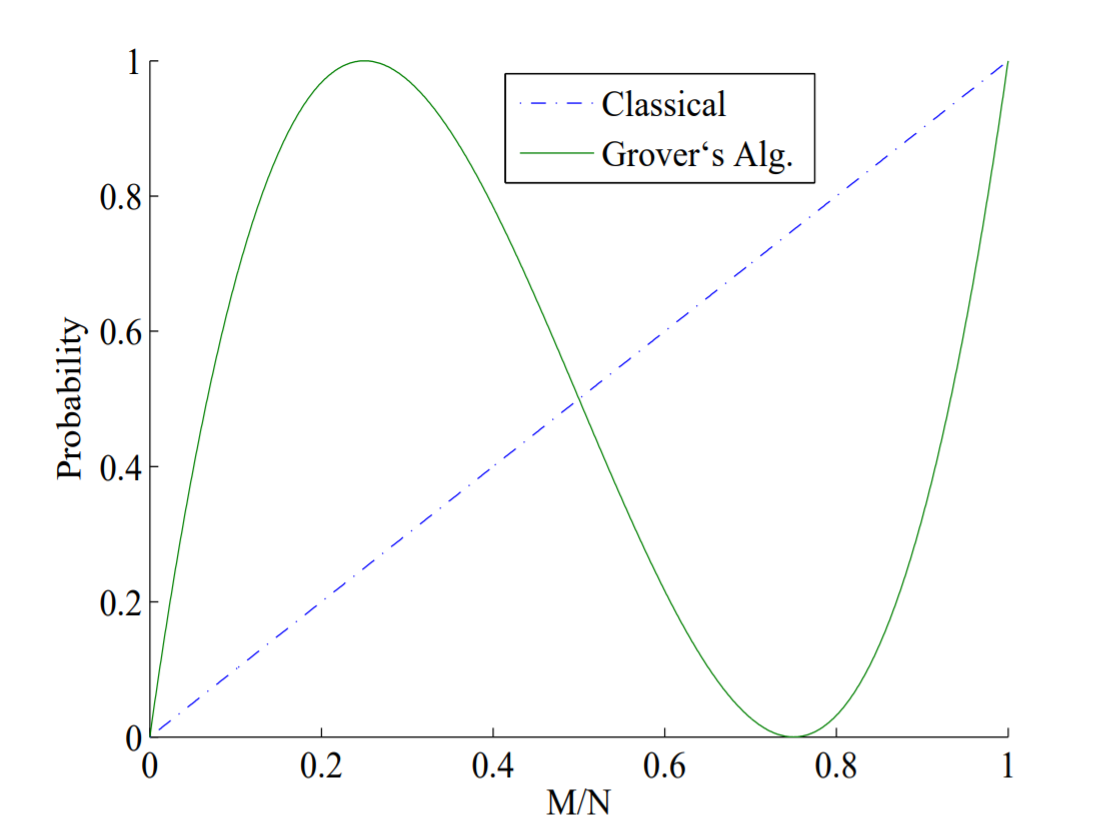
\includegraphics[scale=0.5]{GroverMultipleMatchesRandom.png}
	\caption{Probability of success $P^{Classical}$, $P^{Grover}$ as a function of $\frac{M}{N}$}
\end{figure}

We can see from figure YYY that Grover’s algorithm solves the case where $M = \frac{N}{4}$ with certainty.
The probability of success of Grover’s algorithm will be below one-half for M > $\frac{N}{2}$ and will fail
with certainty for $M = \frac{3}{4}$. The probability of success of the classical guess technique is always over that of Grover’s algorithm for M > N/2.
Now let's concentrate of how the quantum algorithm behaves when iterate following (4).

\begin{figure}[h]
	\centering
	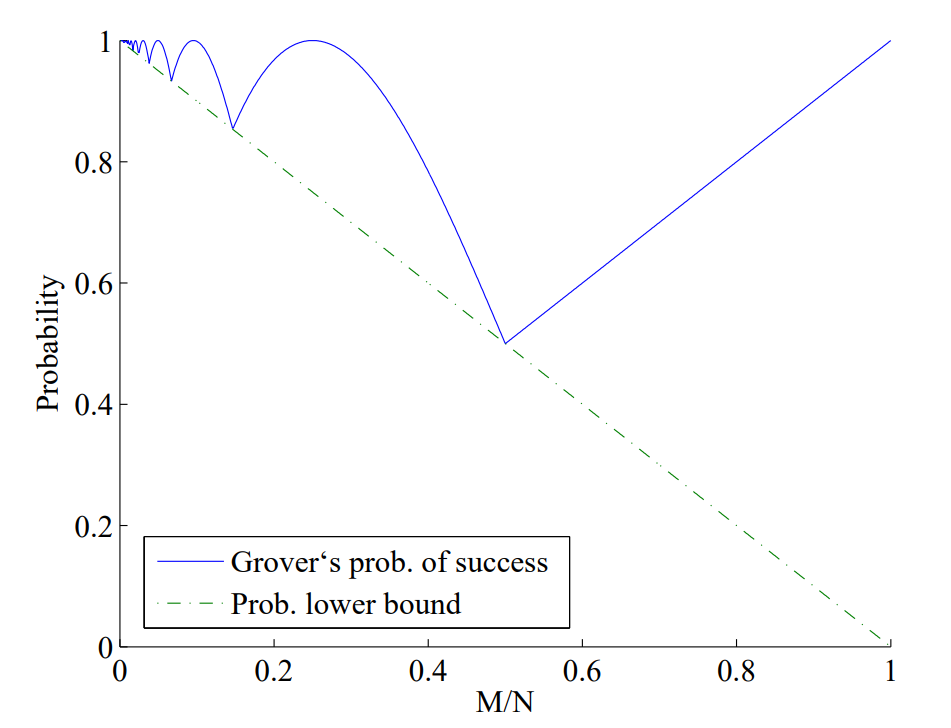
\includegraphics[scale=0.5]{GroverMultipleMatches.png}
	\caption{Probability of success $P^{Classical}$, $P^{Grover}$ as a function of $\frac{M}{N}$}
\end{figure}

As we can see from figure YYY the algorithm behaves better. The minimum probability of finding the correct result is $0.5$ when $\frac{M}{N}$ is equal to $0.5$. When $\frac{M}{N}$ is less then $0.25$ the algorithm have an high probability of finding a result but when $\frac{M}{N}$ is more than $0.5$ tha algorithm behave as a classical random guesser.

\end{document}

\newpage
